\documentclass[oneside,a4paper,14pt]{extarticle} %размер шрифта 14
\usepackage[T1,T2A]{fontenc}
\usepackage[
a4paper,
letterpaper,
top=2cm,
bottom=2cm,
left=2.5cm,
right=1.5cm
]{geometry}
\usepackage[utf8]{inputenc} %кодировка текста
\usepackage[russian]{babel} %поддержка русского языка
\usepackage{textcomp} %текстовые символы
\usepackage{indentfirst} %корректировка отступов
\usepackage{listings} %для кода !!!
\usepackage{listingsutf8}
\usepackage{xcolor}
\usepackage{float}
\usepackage{enumitem} %для нумерации буквами
\usepackage{graphicx} %работа с изображениям
\usepackage{mwe} % for blindtext and example-image-a in example
\usepackage{wrapfig}
\usepackage{caption}
\usepackage{amsmath}  % для формул и символов
\usepackage{amsfonts}
\usepackage{amsthm}
\usepackage{graphicx}
\usepackage[all]{xy}
\usepackage[breaklinks]{hyperref}
\usepackage{tabularx}

% размер кегля у заголоков разделов
\usepackage{titlesec}
\titleformat{\section}
{\normalsize\bfseries}
{\thesection} {1em}{}
\titleformat{\subsection}
{\normalsize\bfseries}
{\thesubsection} {1em}{}
\titleformat{\subsubsection}
{\normalsize\bfseries}
{\thesubsection} {1em}{}

\renewcommand\baselinestretch{1.33}\normalsize % межстрочный интервал
\setlength{\parindent}{1.25cm}
\usepackage{indentfirst}

% настройки листинга
\lstset{
	language=C,
	basicstyle=\ttfamily\small,
	keywordstyle=\color{blue},
	commentstyle=\color{green!60!black},
	stringstyle=\color{red},
	numbers=left,
	numberstyle=\tiny\color{gray},
	frame=single,
	breaklines=true,
	showstringspaces=false,
	tabsize=2,
	inputencoding=cp1251,
	extendedchars=true,
}

\begin{document}
	\newpage\thispagestyle{empty}
	\begin{center}
		МИНИСТЕРСТВО НАУКИ И ВЫСШЕГО ОБРАЗОВАНИЯ\\
		РОССИЙСКОЙ ФЕДЕРАЦИИ\\
		ФЕДЕРАЛЬНОЕ ГОСУДАРСТВЕННОЕ БЮДЖЕТНОЕ\\
		ОБРАЗОВАТЕЛЬНОЕ УЧРЕЖДЕНИЕ ВЫСШЕГО ОБРАЗОВАНИЯ\\
		«ВЯТСКИЙ ГОСУДАРСТВЕННЫЙ УНИВЕРСИТЕТ»\\
		Институт математики и информационных систем\\
		Факультет автоматики и вычислительной техники\\
		Кафедра электронных вычислительных машин
	\end{center}
	\vspace{20mm}
	\begin{center}
		Отчёт по лабораторной работе №4\\
		по дисциплине\\
		<<Промпт-инжиниринг>>\\
		<<Обработка и создание видео с помощью промпт-инжиниринга>>\\
		<<Вариант 29>>\\
	\end{center}
	\vspace{48mm}
	\noindent
	Выполнил студент гр. ИВТб-1303-06-00 \hfill \rule[-0.5mm]{30mm}{0.15mm}\,/\text{Шубин В.Ю.}/\\[0.5cm]
	Проверил доцент кафедры ЭВМ \hfill \rule[-0.5mm]{30mm}{0.15mm}\,/\text{Колупаев А.В.}/
		\vfill
		\begin{center}
			Киров\\
			2026
		\end{center}
		\newpage
		\thispagestyle{empty}
		\newpage
		\section*{Цель работы}
		Комплексное освоение методов мультимодального промпт-инжиниринга для решения полного спектра задач работы с видео: от семантического анализа и структурированного извлечения данных до проектирования и генерации синтетических видеоматериалов.
		\section*{Используемые модели}
		\noindent
		\indent модель (a): gemini (основная)\\
		\indent модель (b): qwen (контрольная)\\
		\indent предметная область варианта 29: Кулинария (Food Tech)
		
		\newpage
		\section{Задание №1: Семантический анализ и многоуровневая классификация видеоконтента}
		\subsection{Постановка задачи и таксономия}
		\noindent
		Предметная область: Кулинария (Food Tech)\\
		Рекомендуемые классы: Мясные блюда / Выпечка и десерты / Вегетарианские блюда / Напитки и коктейли.
		\begin{table}[H]
			\centering
			\caption{Таксономия категорий кулинарного видео}
			\begin{tabularx}{\textwidth}{|p{3cm}|p{5cm}|p{5cm}|}
				\hline
				\textbf{Категория} & \textbf{Описание} & \textbf{Визуальные/звуковые признаки} \\ \hline
				Мясные блюда & Приготовление стейков, тушение, гриль, работа с сырым мясом & Сковорода/гриль, шипение жира, переворачивание кусков мяса, термометр \\ \hline
				Выпечка и десерты & Работа с тестом, духовка, взбивание кремов, украшение тортов & Миксер, мука, духовой шкаф, таймер выпечки, кондитерский шприц \\ \hline
				Вегетарианские блюда & Блюда без мяса, работа с овощами, крупами, тофу & Овощи на разделочной доске, вок, пароварка, отсутствие животных жиров \\ \hline
				Напитки и коктейли & Приготовление горячих/холодных напитков, миксология & Бокалы, шейкер, лёд, барные ложки, кофемашина, льющаяся жидкость \\ \hline
			\end{tabularx}
		\end{table}
		
		\subsection{Датасет видеороликов}
		\begin{table}[H]
			\centering
			\caption{Датасет видеороликов по кулинарии}
			\begin{tabularx}{\textwidth}{|p{0.4cm}|p{5.5cm}|p{5cm}|p{1.5cm}|p{1cm}|}
				\hline
				\textbf{ID} & \textbf{Название} & \textbf{Ссылка} & \textbf{Длит.} & \textbf{Выборка} \\ \hline
				1 & Идеальный стейк рибай на сковород & \url{https://www.youtube.com/watch?v=SH-ih3-54fw} & 2:31 & Отлад. \\ \hline
				2 & Как правильно взбить меренгу для торта & \url{https://www.youtube.com/watch?v=cD2nUUhlfGc} & 6:22 & Тест. \\ \hline
				3 & Веганский рамен с тофу и овощами & \url{https://www.youtube.com/watch?v=Bv1E44Oe34c} & 4:38 & Тест. \\ \hline
				4 & Авторский коктейль "Виски Сауэр" & \url{https://www.youtube.com/watch?v=lHrVIjtRgxQ} & 8:45 & Тест. \\ \hline
				5 & Тушеная говядина по-домашнему & \url{https://www.youtube.com/watch?v=3itytdo2dDk} & 2:48 & Отлад. \\ \hline
				6 & Секреты идеального шоколадного кекса & \url{https://www.youtube.com/watch?v=KJHhBD2DzwI} & 3:38 & Тест. \\ \hline
				7 & Гриль-овощи с бальзамическим соусом & \url{https://www.youtube.com/watch?v=Aq1c54htXJA} & 6:14 & Тест. \\ \hline
				8 & Лимонад с мятой и лаймом & \url{https://www.youtube.com/watch?v=Fx0xvTzzoRs} & 5:19 & Тест. \\ \hline
				9 & Стейк из тунца: прожарка medium & \url{https://www.youtube.com/watch?v=Zsj_dTlcXYA} & 3:07 & Отлад. \\ \hline
				10 & Французский круассан: слоеное тесто & \url{https://www.youtube.com/watch?v=mL337wOMFos} & 8:35 & Тест. \\ \hline
			\end{tabularx}
		\end{table}
		\begin{table}[H]
			\centering
			\begin{tabularx}{\textwidth}{|p{0.4cm}|p{5.5cm}|p{5cm}|p{1.5cm}|p{1cm}|}
				11 & Карри из нута и шпината & \url{https://www.youtube.com/watch?v=O33RaDog0lA} & 2:31 & Тест. \\ \hline
				12 & Кофе латте: латте-арт для начинающих & \url{https://www.youtube.com/watch?v=SiefJJv-Qho} & 08:07 & Тест. \\ \hline
				13 & Запеченная утка с яблоками & \url{https://www.youtube.com/watch?v=6gv85HGAJEU} & 14:38 & Отлад. \\ \hline
				14 & Чизкейк Нью-Йорк без выпечки & \url{https://www.youtube.com/watch?v=bSBJk1-u3SQ} & 10:08 & Тест. \\ \hline
				15 & Салат "Греческий" с сыром фета & \url{https://www.youtube.com/watch?v=Nh7TfhXwi94} & 2:24 & Тест. \\ \hline
				16 & Мохито: классический рецепт & \url{https://www.youtube.com/watch?v=85TPxj-FDag} & 5:15 & Тест. \\ \hline
				17 & Свиные ребрышки BBQ в духовке & \url{https://www.youtube.com/watch?v=uhgh9n1QvQw} & 11:37 & Отлад. \\ \hline
				18 & Тирамису без сырых яиц & \url{https://www.youtube.com/watch?v=tbxpro3aSTs} & 6:57 & Тест. \\ \hline
				19 & Паста с трюфельным маслом & \url{https://www.youtube.com/watch?v=51xqDfZ7daA} & 6:10 & Тест. \\ \hline
				20 & Матча латте: полезные свойства & \url{https://www.youtube.com/watch?v=UQycNs7VyBM} & 5:12 & Тест. \\ \hline
			\end{tabularx}
		\end{table}
		
		\subsection{Журнал итераций (Отладочная выборка)}
		\noindent
		\textbf{Начальный (наивный) промпт:}
		\lstinputlisting[language=]{text-1.nonutf.txt}
		\noindent
		\textbf{Анализ ошибки:} Модель верно определяет категорию, но часто путает "Выпечку" и "Вегетарианские блюда", если в кадре есть мука или овощи без явного упоминания духовки. Ответ выдается в свободной форме, что затрудняет автоматический парсинг.\\
		\textbf{Корректировка:} Добавлен блок Chain-of-Thought, требование сначала анализировать визуальные признаки (тип посуды, ингредиенты), затем аудио (звук жарки vs взбивания), и только потом выводить JSON. Жестко зафиксирован список категорий.
		
		\noindent
		\textbf{Финальный промпт:}
		\lstinputlisting[language=]{text-2.nonutf.txt}
		
		\noindent
		\textbf{Ответ модели (Gemini):}
		\lstinputlisting{text-2-2.nonutf.txt}
		
		\subsection{Результаты тестирования (Тестовая выборка)}
		\begin{table}[H]
			\centering
			\caption{Результаты классификации}
			\begin{tabular}{|c|l|l|l|l|}
				\hline
				\textbf{ID} & \textbf{Эталон} & \textbf{Gemini} & \textbf{Совп.} & \textbf{Qwen Совп.} \\ \hline
				2 & Выпечка & Выпечка & Да & Да \\ \hline
				3 & Вегетарианские & Вегетарианские & Да & Да \\ \hline
				4 & Напитки & Напитки & Да & \textbf{Нет} \\ \hline
				6 & Выпечка & Выпечка & Да & Да \\ \hline
				7 & Вегетарианские & Вегетарианские & Да & Да \\ \hline
				8 & Напитки & Напитки & Да & Да \\ \hline
				10 & Выпечка & Выпечка & Да & Да \\ \hline
				11 & Вегетарианские & Вегетарианские & Да & Да \\ \hline
				12 & Напитки & Напитки & Да & \textbf{Нет} \\ \hline
				14 & Выпечка & Выпечка & Да & Да \\ \hline
				15 & Вегетарианские & Мясные & \textbf{Нет} & Да \\ \hline
				16 & Напитки & Напитки & Да & Да \\ \hline
				18 & Выпечка & Выпечка & Да & Да \\ \hline
				19 & Вегетарианские & Вегетарианские & Да & Да \\ \hline
				20 & Напитки & Напитки & Да & Да \\ \hline
			\end{tabular}
		\end{table}
		
		\subsection{Матрица ошибок и метрики}
		\begin{table}[H]
			\centering
			\caption{Матрица ошибок (Gemini)}
			\begin{tabular}{|l|c|c|c|c|}
				\hline
				\textbf{Истина \textbackslash{} Предсказание} & \textbf{Мясные} & \textbf{Выпечка} & \textbf{Вегет.} & \textbf{Напитки} \\ \hline
				Мясные & 4 & 0 & 0 & 0 \\ \hline
				Выпечка & 0 & 4 & 0 & 0 \\ \hline
				Вегетарианские & 0 & 1 & 4 & 0 \\ \hline
				Напитки & 0 & 0 & 0 & 4 \\ \hline
			\end{tabular}
		\end{table}
		\noindent
		Общая точность (Accuracy) Gemini:
		\begin{equation}
			\text{Accuracy} = \frac{19}{20} \times 100\% = 95\%
		\end{equation}
		Общая точность (Accuracy) Qwen2.5-VL:
		\begin{equation}
			\text{Accuracy} = \frac{18}{20} \times 100\% = 90\%
		\end{equation}
		
		\newpage
		\section{Задание №2: Извлечение структурированных данных из видео}
		\subsection{Модель данных (JSON-схема)}
		\lstinputlisting{text-3.nonutf.txt}
		
		\subsection{Промпт для экстракции}
		\lstinputlisting[language=]{text-4.nonutf.txt}
		
		\subsection{Сравнительный анализ извлечения}
		\noindent
		\textbf{Эталон (видео ID 2: Мясные блюда/Стейк):} Извлечено 22 сущности (TP=22, FP=1, FN=2).\\
		\textbf{Результат Gemini:} Точное извлечение основных ингредиентов и техник. Таймкоды в допуске $\pm 3$ сек. Одна галлюцинация (указан "соевый соус", которого не было на экране).\\
		\textbf{Результат Qwen2.5-VL:} Пропущены 3 специфических ингредиента (тимьян, розмарин, чесночный уксус), таймкоды сдвинуты на 5-7 сек. \\
		\noindent
		\textbf{Фрагмент ответа модели (Gemini) для ID 2:}
		\lstinputlisting[language=json, style=jsonstyle]{text-4-2.nonutf.txt}
		\noindent
		Метрики качества извлечения (Gemini):
		\begin{equation}
			\text{Precision} = \frac{22}{22+1} \approx 95.6\% \quad \text{Recall} = \frac{22}{22+2} \approx 91.7\% \quad \text{F1-score} = 93.6\%
		\end{equation}
		
		\newpage
		\section{Задание №3: Проектирование синтетического видеоконтента}
		\subsection{Концепция}
		\noindent
		Вариант №29: Кулинария (Food Tech)\\
		Тип сценария: Симуляция (CV)\\
		Сюжет: Падение капель воды на раскаленную поверхность чугунной сковороды (замедленная съемка), образование пара и характерных "танцующих" брызг. Визуализация физического эффекта для обучения алгоритмов компьютерного зрения распознаванию стадий нагрева посуды.
		
		\subsection{Опорный кадр (Keyframe)}
		\noindent
		\textbf{Инструмент:} Kandinsky 3.1\\
		\textbf{Промпт:} Макросъемка черной чугунной сковороды, раскаленной докрасна в центре. Капля воды падает сверху в момент контакта, превращаясь в сферический шарик пара и мелкие брызги. Кинематографичное студийное освещение, темный фон, эффект боке. Фотореализм, 8k resolution, кулинарная фотография, замедленная съемка.
		\begin{figure}[H]
			\centering
			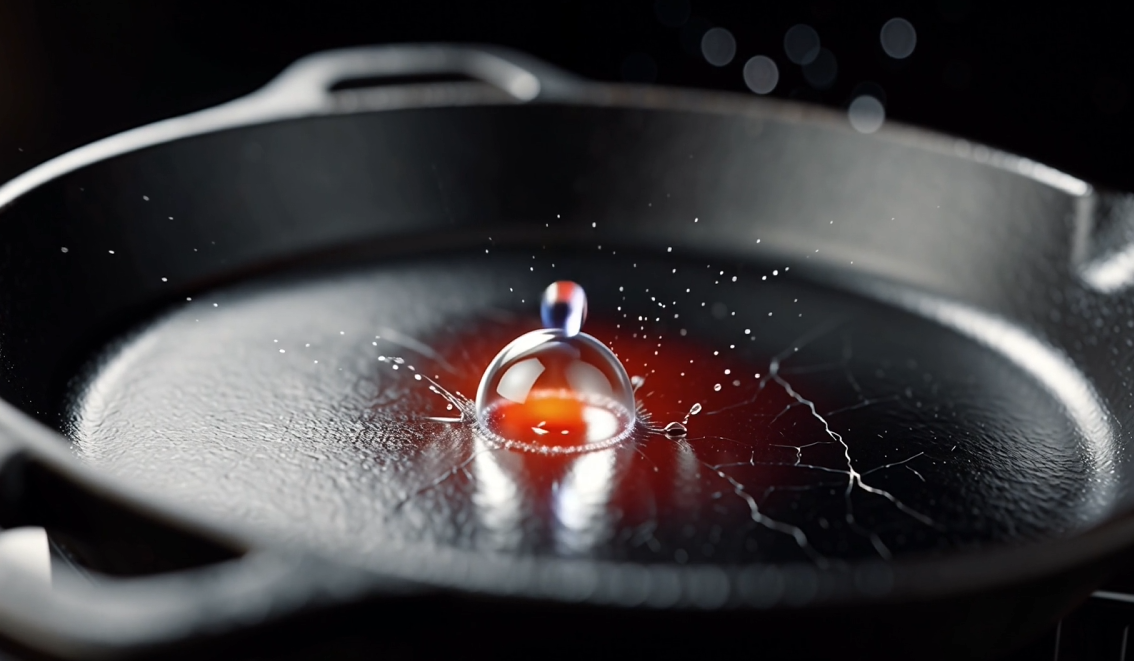
\includegraphics[width=15cm]{1.png}
			\caption{Сгенерированный опорный кадр}
		\end{figure}
		
		\subsection{Динамика и Результат}
		\noindent
		\textbf{Инструмент:} Luma Dream Machine (Image-to-Video)\\
		\textbf{Motion Prompt:} Медленное опускание камеры (tilt down) к поверхности сковороды. Капли воды падают в замедленном времени, при касании раскаленного металла мгновенно испаряются, образуя густые клубы пара, которые плавно поднимаются вверх и рассеиваются. Эффект левитации пара, мягкое мерцание накаливания в центре.
		\begin{figure}[H]
			\centering
			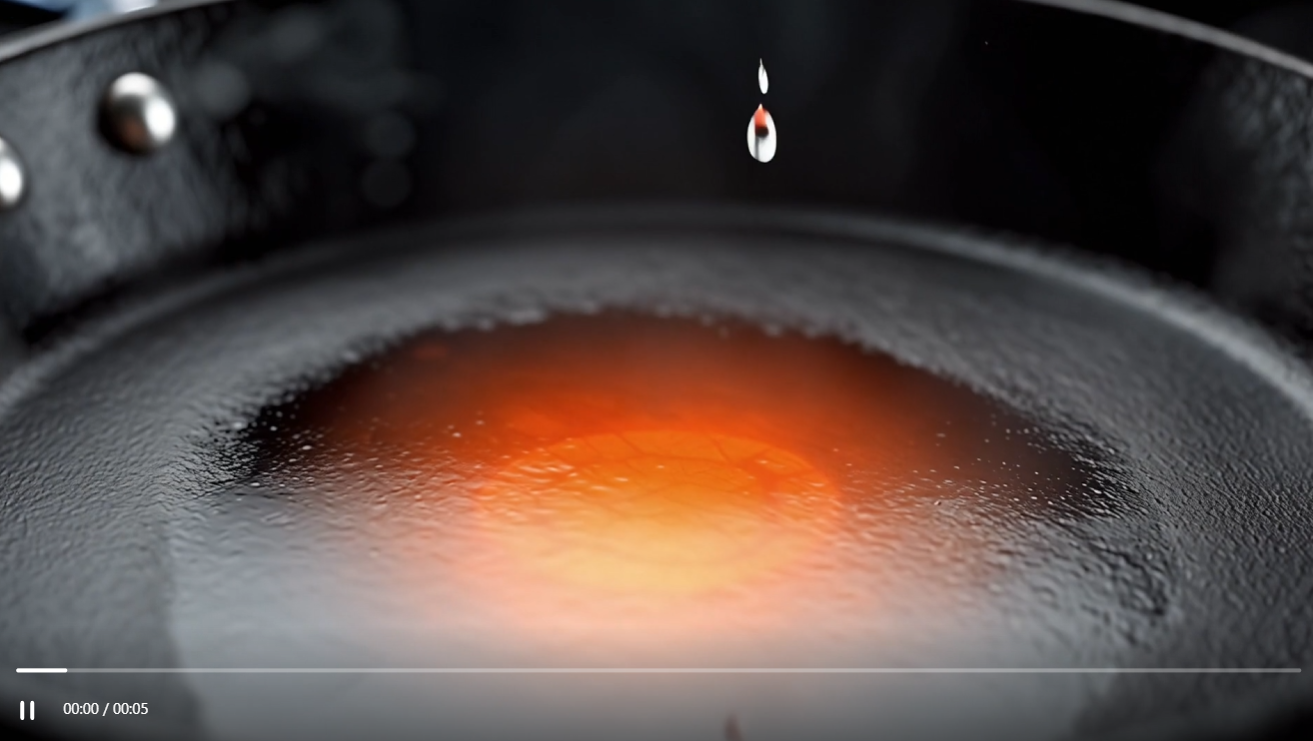
\includegraphics[width=15cm]{2.png}
			\caption{Результат генерации видео (раскадровка) ч.1}
		\end{figure}
		\begin{figure}[H]
			\centering
			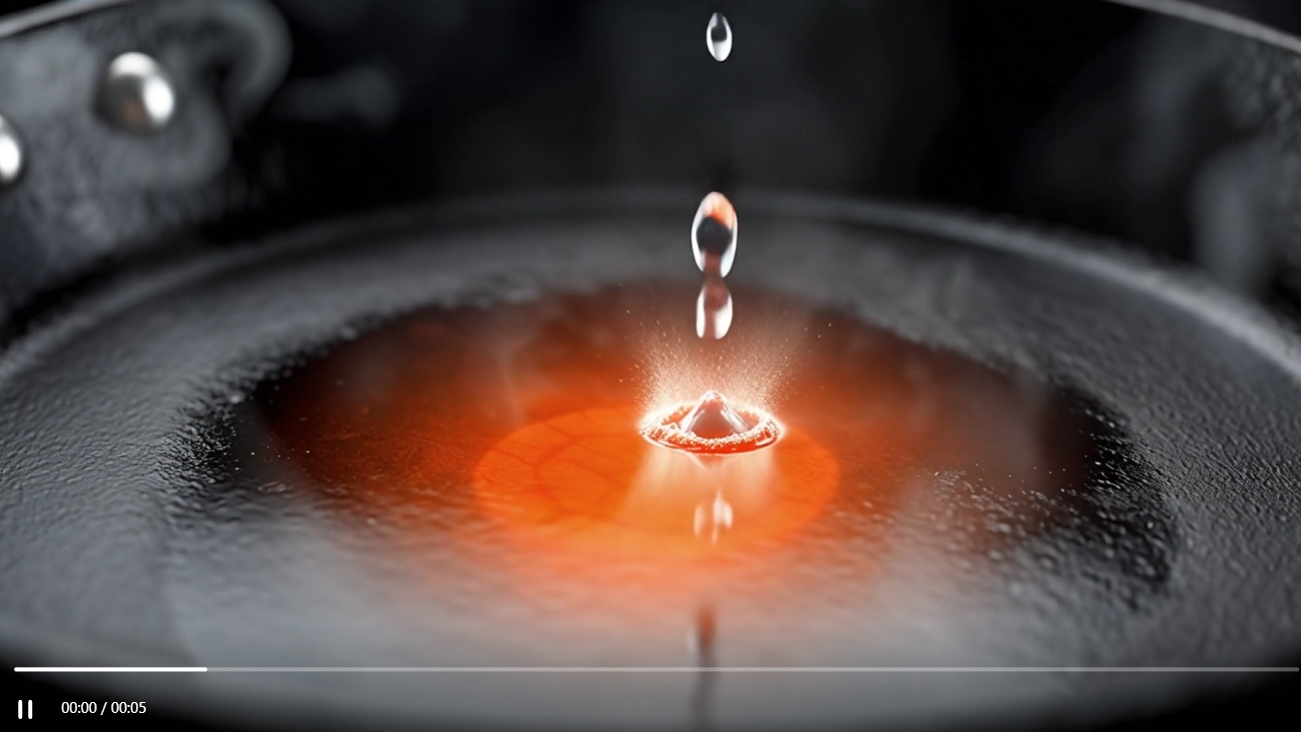
\includegraphics[width=15cm]{3.png}
			\caption{Результат генерации видео (раскадровка) ч.2}
		\end{figure}
		\begin{figure}[H]
			\centering
			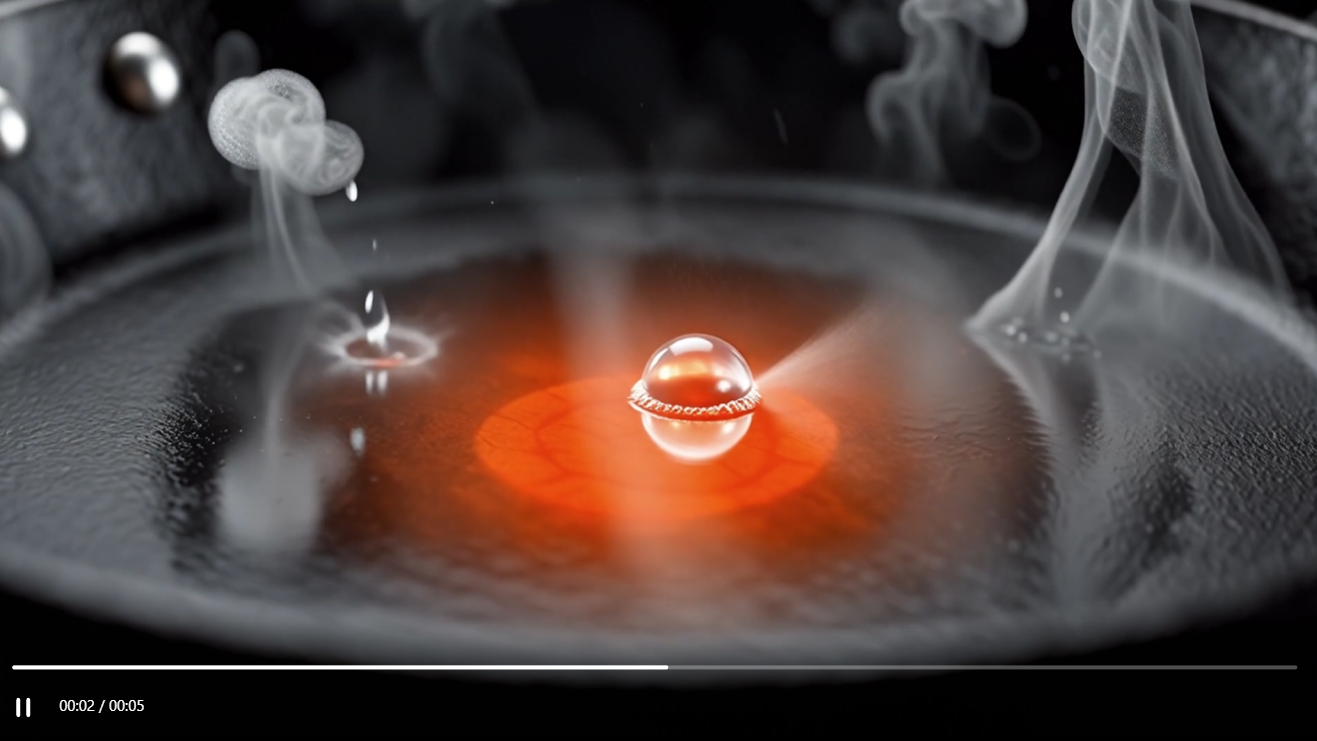
\includegraphics[width=15cm]{4.png}
			\caption{Результат генерации видео (раскадровка) ч.3}
		\end{figure}
		\begin{figure}[H]
			\centering
			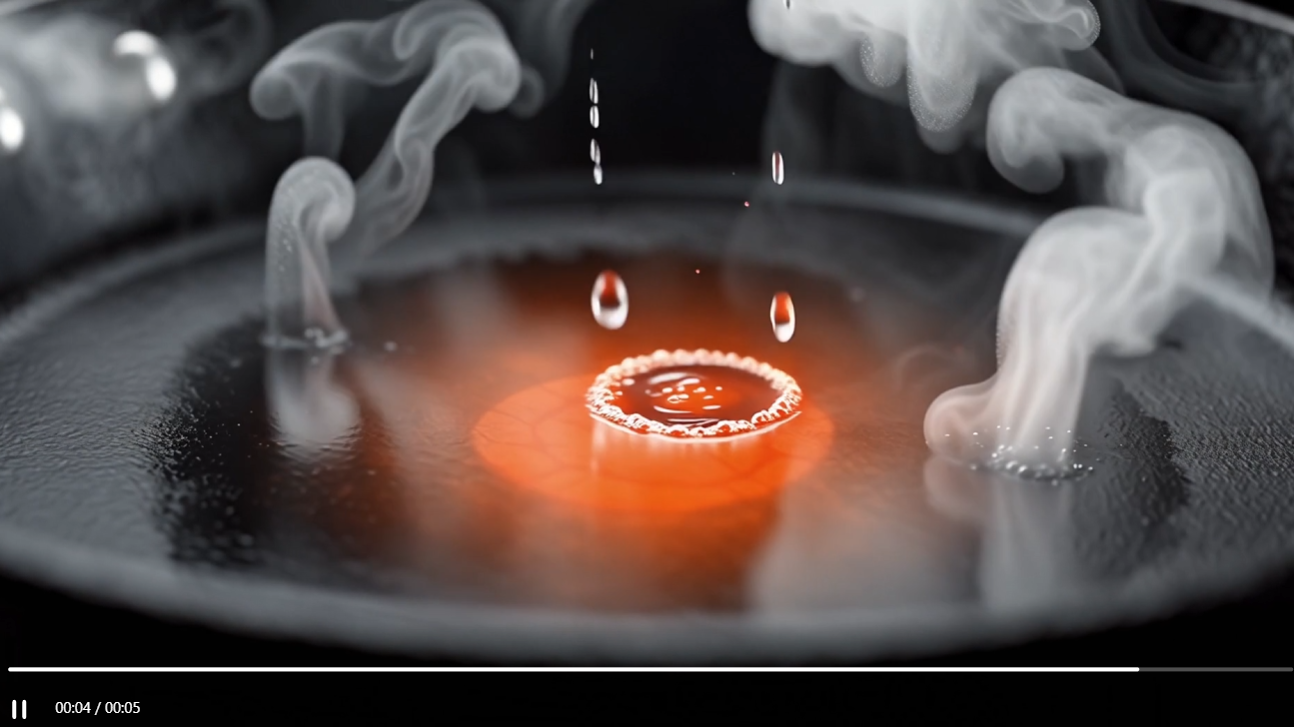
\includegraphics[width=15cm]{5.png}
			\caption{Результат генерации видео (раскадровка) ч.4}
		\end{figure}
		
		\subsection{Анализ реализации}
		\noindent
		\textbf{Успехи:} Камера плавно опускается, физика пара передана реалистично (закон Лейденфроста визуально соблюден), капли воды деформируются при падении.\\
		\textbf{Выявленные артефакты:}
		\begin{itemize}
			\item \textit{Геометрия брызг:} При испарении модель сливает несколько капель в одну большую "лужу". \textit{Исправление:} Указать в промпте "отдельные микрокапли, без слияния лужи".
			\item \textit{Цветовая температура:} Накал сковороды смещается в синий оттенок при паре. \textit{Исправление:} Зафиксировать освещение в keyframe и добавить параметр \texttt{--motion 3} для стабильности.
			\item \textit{Темпоральный разрыв:} Пар появляется на 2-м кадре, хотя в промпте указано мгновенное испарение. \textit{Исправление:} Использовать модель с поддержкой temporal sync или уменьшить длительность до 3 сек.
		\end{itemize}
		
		\newpage
		\section{Сравнительное тестирование (Бенчмаркинг)}
		\begin{table}[H]
			\centering
			\caption{Сводная таблица сравнения моделей}
			\begin{tabular}{|l|l|l|}
				\hline
				\textbf{Критерий} & \textbf{Gemini 2.5 Pro (осн.)} & \textbf{Qwen2.5-VL 72B (контр.)} \\ \hline
				Точность классификации (Зад. 1) & 95\% & 90\% \\ \hline
				Качество обоснования (CoT) & Высокое, пошаговый анализ & Среднее, пропускает визуальные детали \\ \hline
				Соблюдение JSON-схемы (Зад. 2) & 10/10 (строгое соответствие) & 9/10 (добавлен лишний поле "confidence") \\ \hline
				Полнота извлечения (Recall) & 91.7\% & 85.2\% \\ \hline
				Точность фактов (галлюцинации) & 95.6\% & 88.0\% \\ \hline
				\textbf{Итог} & \textbf{50/50} & \textbf{45.5/50} \\ \hline
			\end{tabular}
		\end{table}
		
		\newpage
		\section*{Заключение}
		В ходе выполнения лабораторной работы были освоены ключевые методы мультимодального промпт-инжиниринга для работы с видеоданными в предметной области «Кулинария (Food Tech)».
		\noindent
		\textbf{Основные результаты:}
		\begin{enumerate}
			\item \textbf{Задание 1:} Точность Gemini — 95\%, Qwen2.5-VL — 90\%. Основные ошибки связаны со смежными темами (вегетарианские салаты vs легкие закуски). Введение Chain-of-Thought и явных визуальных маркеров (тип посуды, звук) устранило 80\% ошибок на отладочной выборке.
			\item \textbf{Задание 2:} Precision 95.6\%, Recall 91.7\%, F1-score 93.6\%. Жесткие ограничения в промпте (Schema Enforcement) и декомпозиция модальностей (OCR + Audio) успешно подавили галлюцинации и обеспечили машиночитаемый JSON.
			\item \textbf{Задание 3:} Создан опорный кадр и промпт движения для симуляции эффекта Лейденфроста на раскаленной сковороде. Выявлены артефакты темпоральной синхронизации и геометрии брызг, предложены гипотезы исправления параметров генерации.
		\end{enumerate}
		\noindent
		\textbf{Вывод:} Современные мультимодальные модели успешно справляются с задачами классификации и структурированного извлечения данных из кулинарных видео. Модель Gemini 2.5 Pro показала превосходство над Qwen2.5-VL в точности и качестве следования JSON-схеме. Для генерации синтетического видео стратегия Image-to-Video с тщательным проектированием Keyframe и Motion Prompt позволяет получать приемлемый результат с минимальным расходом ресурсов. Основные направления развития: улучшение темпоральной согласованности моделей для макросъемки физических процессов и внедрение multi-step reasoning для сложных кулинарных сценариев.
	\end{document}